\section{Data and exploratory analysis}
\label{sec:data_eda}

We evaluate two F3 settings. In the first, clay volume is reconstructed in a
held-out well. In the second, porosity in one well is reconstructed from
gamma ray alone.

\subsection{Field settings and benchmark provenance}
\label{subsec:field_settings}

The experiments use the processed F3 well-log curves of
\citet{zhang2025rockphysicslogs}; no new field data were acquired. We use the
FS2--FS6 intervals of F02-1, F03-2, F03-4, and F06-1. Sonic and gamma ray are
available in all wells; density is measured in F02-1/F03-2 and predicted in
F03-4/F06-1. Porosity is density-derived and clay volume $V_c$ is
Larionov-derived from
gamma ray; further geological and processing details are given in the source
study.

The cross-well benchmark reconstructs $V_c$ from $30~\mathrm{dB}$ noisy logs,
using F02-1, F03-2, and F06-1 for development and F03-4 for testing. The
single-well benchmark reconstructs F03-4 porosity from gamma ray alone. In both,
$\boldsymbol{b}$ is obtained by coordinate subsampling of the processed target.
Appendix~\ref{app:lapa_case} provides a limited-sample Lapa permeability case
based on \citet{alvarez2025nonlinear}.

\begin{table}[!htbp]
    \centering
    \caption{Summary of the two F3 benchmarks. The cross-well target $V_c$ is
    derived from gamma ray through the Larionov relation, whereas the
    single-well target is processed porosity.}
    \label{tab:eda_dataset_summary}
    \small
    \adjustbox{max width=\linewidth}{
        \begin{tabular}{lllrrrrrrr}
\toprule
dataset & well & target & n\_rows & depth\_min & depth\_max & target\_mean & target\_std & target\_min & target\_max \\
\midrule
cross\_train & F02-1 & $V_c$ & 165 & 1149.7056 & 1174.6992 & 0.1215 & 0.0407 & 0.0513 & 0.1934 \\
cross\_train & F03-2 & $V_c$ & 811 & 951.9000 & 1073.4000 & 0.1184 & 0.0490 & 0.0393 & 0.2688 \\
cross\_train & F06-1 & $V_c$ & 122 & 1133.1000 & 1151.2500 & 0.1223 & 0.0437 & 0.0427 & 0.2175 \\
cross\_test & F03-4 & $V_c$ & 832 & 946.5000 & 1071.1500 & 0.0824 & 0.0341 & 0.0112 & 0.1699 \\
real\_f03\_gr & F03-4 & Porosity & 1435 & 856.0500 & 1071.1500 & 0.2789 & 0.0142 & 0.2471 & 0.3264 \\
\bottomrule
\end{tabular}

    }
\end{table}

Table~\ref{tab:eda_dataset_summary} summarizes the two settings. Held-out F03-4
has mean $V_c=0.0824$, versus about $0.12$ in the training wells, and
Fig.~\ref{fig:eda_crosswell_distribution} shows a lower-valued but overlapping
distribution. Larger sliding-window steps further reduce training support,
whereas CLP-CSGM can still refine the held-out-well estimate using
$\boldsymbol{b}$ at inference.

\begin{figure}[t]
    \centering
    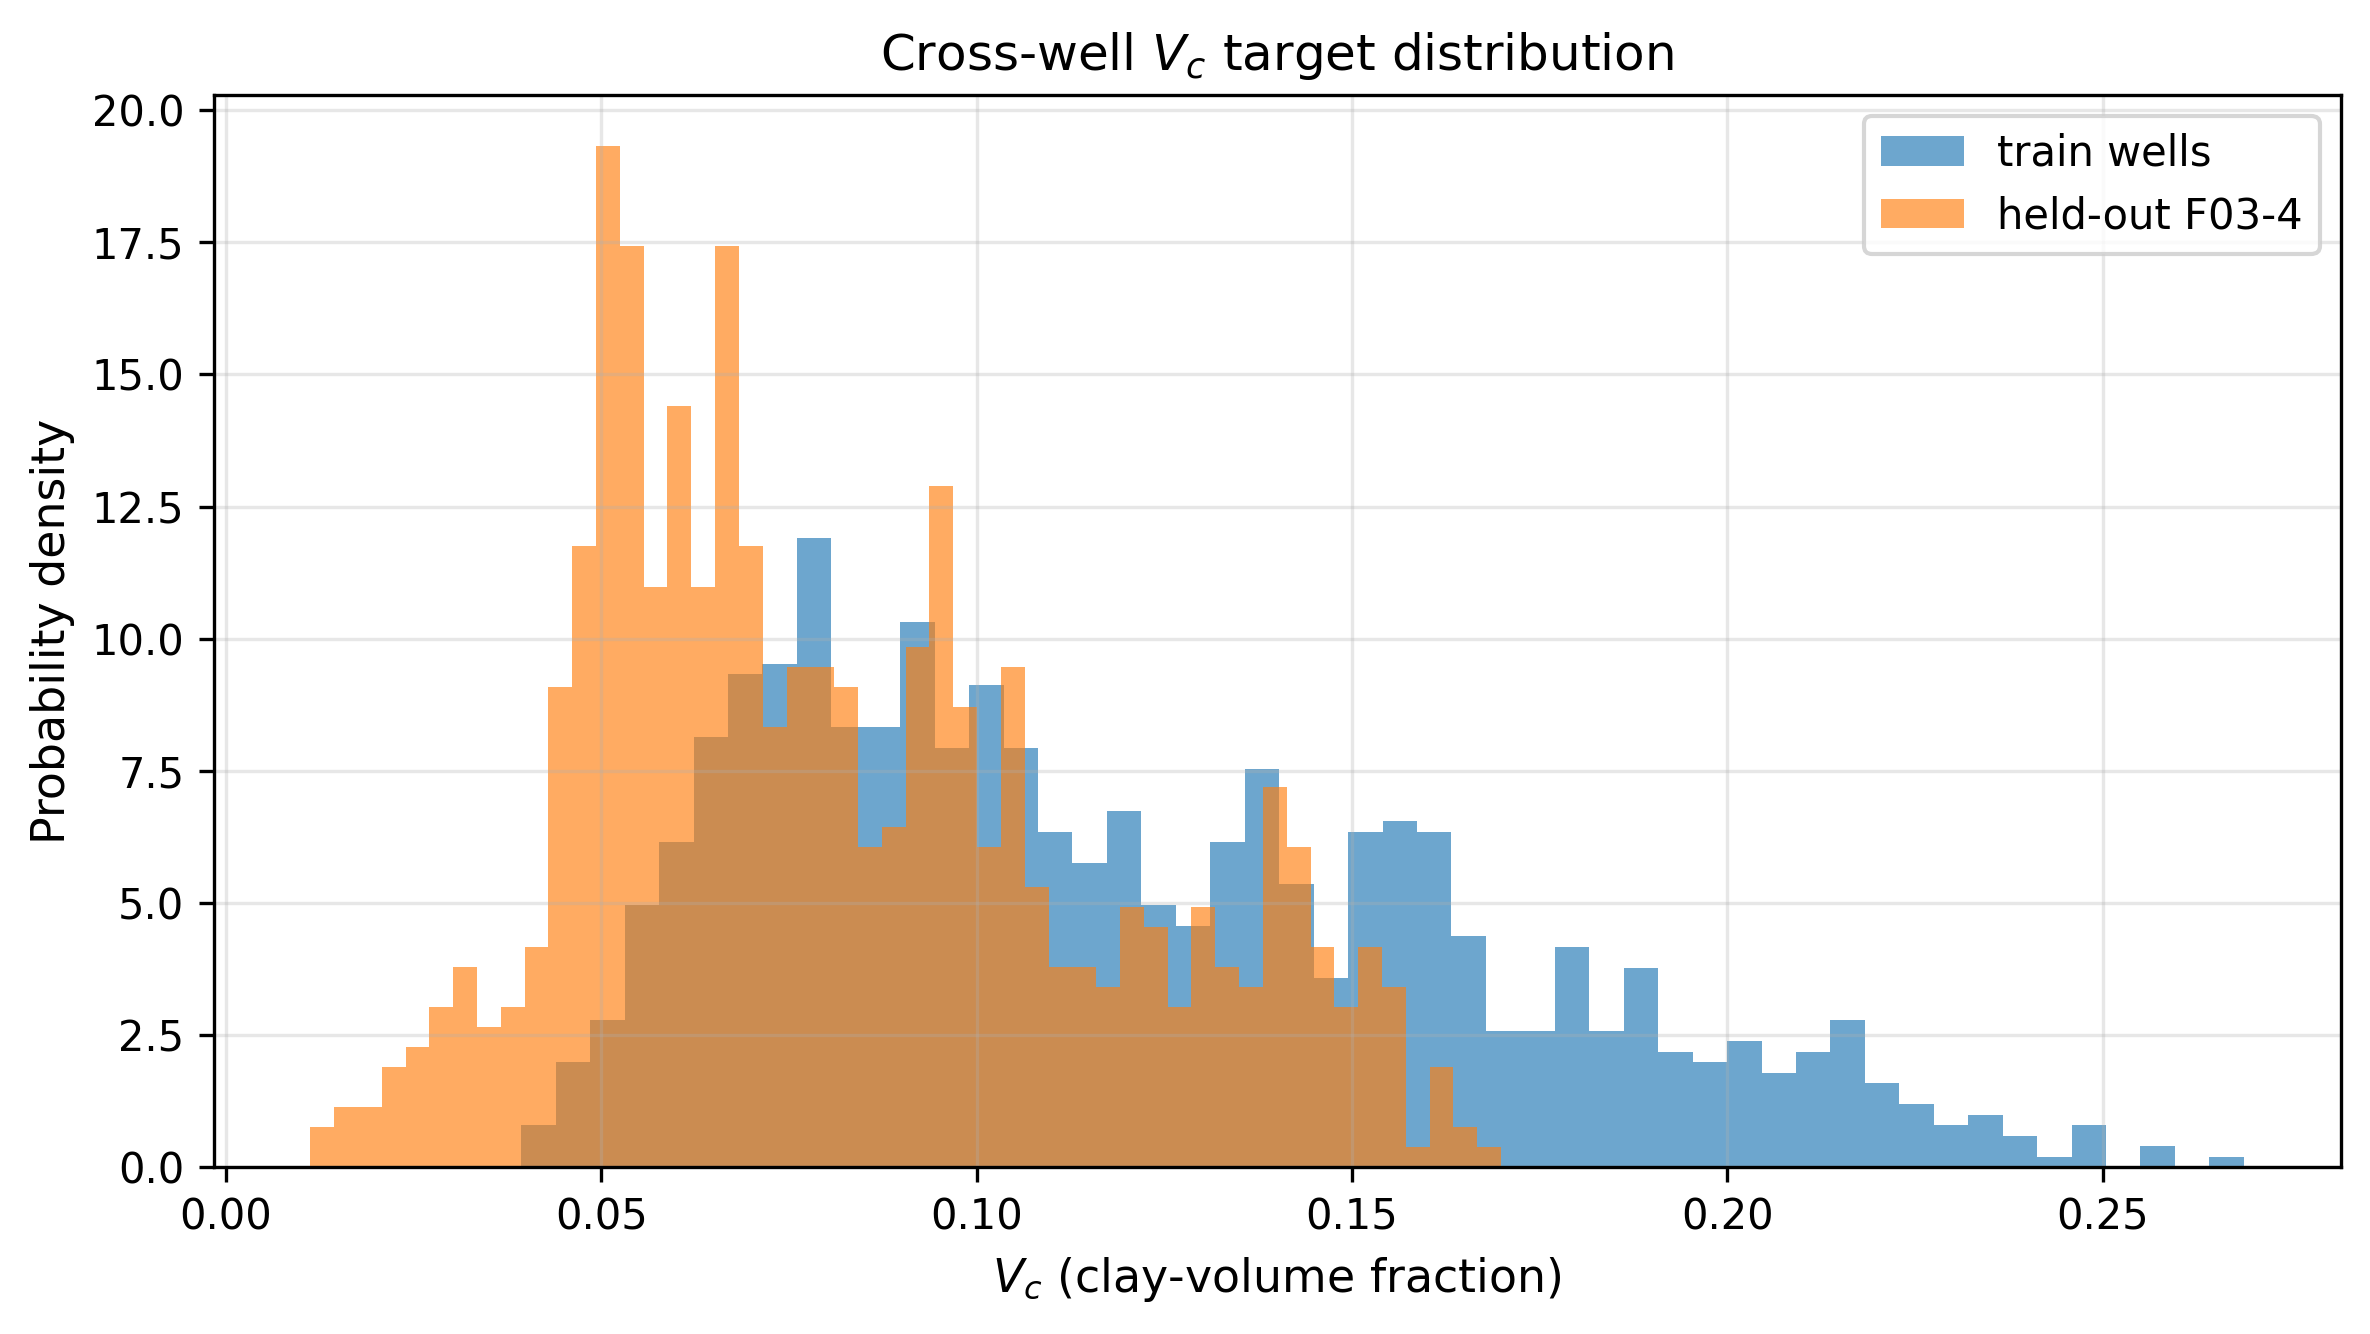
\includegraphics[width=0.68\linewidth]
    {eda_crosswell_vc_distribution.png}
    \caption{Empirical cross-well $V_c$ distributions for the pooled training
    wells and the held-out F03-4 well. The held-out distribution is shifted
    toward lower clay-volume values while retaining partial overlap with the
    training distribution.}
    \label{fig:eda_crosswell_distribution}
\end{figure}

\paragraph{Channel-target correlations and input design.}
Table~\ref{tab:eda_correlations} reports descriptive Pearson correlations used
only to guide input design. Clay volume in this benchmark is computed from gamma ray by the Larionov
relation \citep{zhang2025rockphysicslogs}. The main cross-well input therefore
leaves gamma ray out and uses sonic, density, acoustic impedance, and $V_p$.
With gamma ray included, the model would read the log from which the target
was computed. This is not the usual field interpretation, in which gamma ray
is logged and clay volume is obtained from that relation directly. The
gamma-ray index between the clean and shale endpoints is linear in gamma ray.
The Larionov map from that index to clay volume is not a straight line. When
gamma ray has been logged, that relation is the calculation, and the model is
not a substitute for it. Gamma ray
is put back only in Appendix~\ref{app:crosswell_gr_embargo}, as a check on
the effect of that channel.

\begin{table}[!htbp]
    \centering
    \caption{Pearson correlations between the available input channels and the
    target properties in the cross-well $V_c$ and single-well F03-4 porosity
    benchmarks.}
    \label{tab:eda_correlations}
    \small
    \adjustbox{max width=\linewidth}{
        \begin{tabular}{lllr}
\toprule
dataset & channel & target & pearson\_r \\
\midrule
cross\_train & Sonic & $V_c$ & -0.1642 \\
cross\_train & RHOB & $V_c$ & 0.0807 \\
cross\_train & GR & $V_c$ & 0.9733 \\
cross\_train & AI & $V_c$ & 0.1672 \\
cross\_train & $V_p$ & $V_c$ & 0.1819 \\
cross\_test & Sonic & $V_c$ & -0.1606 \\
cross\_test & RHOB & $V_c$ & -0.0061 \\
cross\_test & GR & $V_c$ & 0.9772 \\
cross\_test & AI & $V_c$ & 0.1330 \\
cross\_test & $V_p$ & $V_c$ & 0.1077 \\
real\_f03 & AC & Porosity & 0.9996 \\
real\_f03 & GR & Porosity & -0.1759 \\
\bottomrule
\end{tabular}

    }
\end{table}

In F03-4, sonic travel time follows the processed porosity almost one to one,
whereas gamma ray is only weakly related to it. Sonic is left out for that
reason. The density curve behind this porosity was itself predicted from sonic
and gamma ray. The test that remains uses gamma ray as the only dense log and
keeps a few values of the porosity curve as measurements. It is not a porosity
interpretation from density, neutron, and sonic together
(Fig.~\ref{fig:eda_f03_profile}).

\begin{figure}[t]
    \centering
    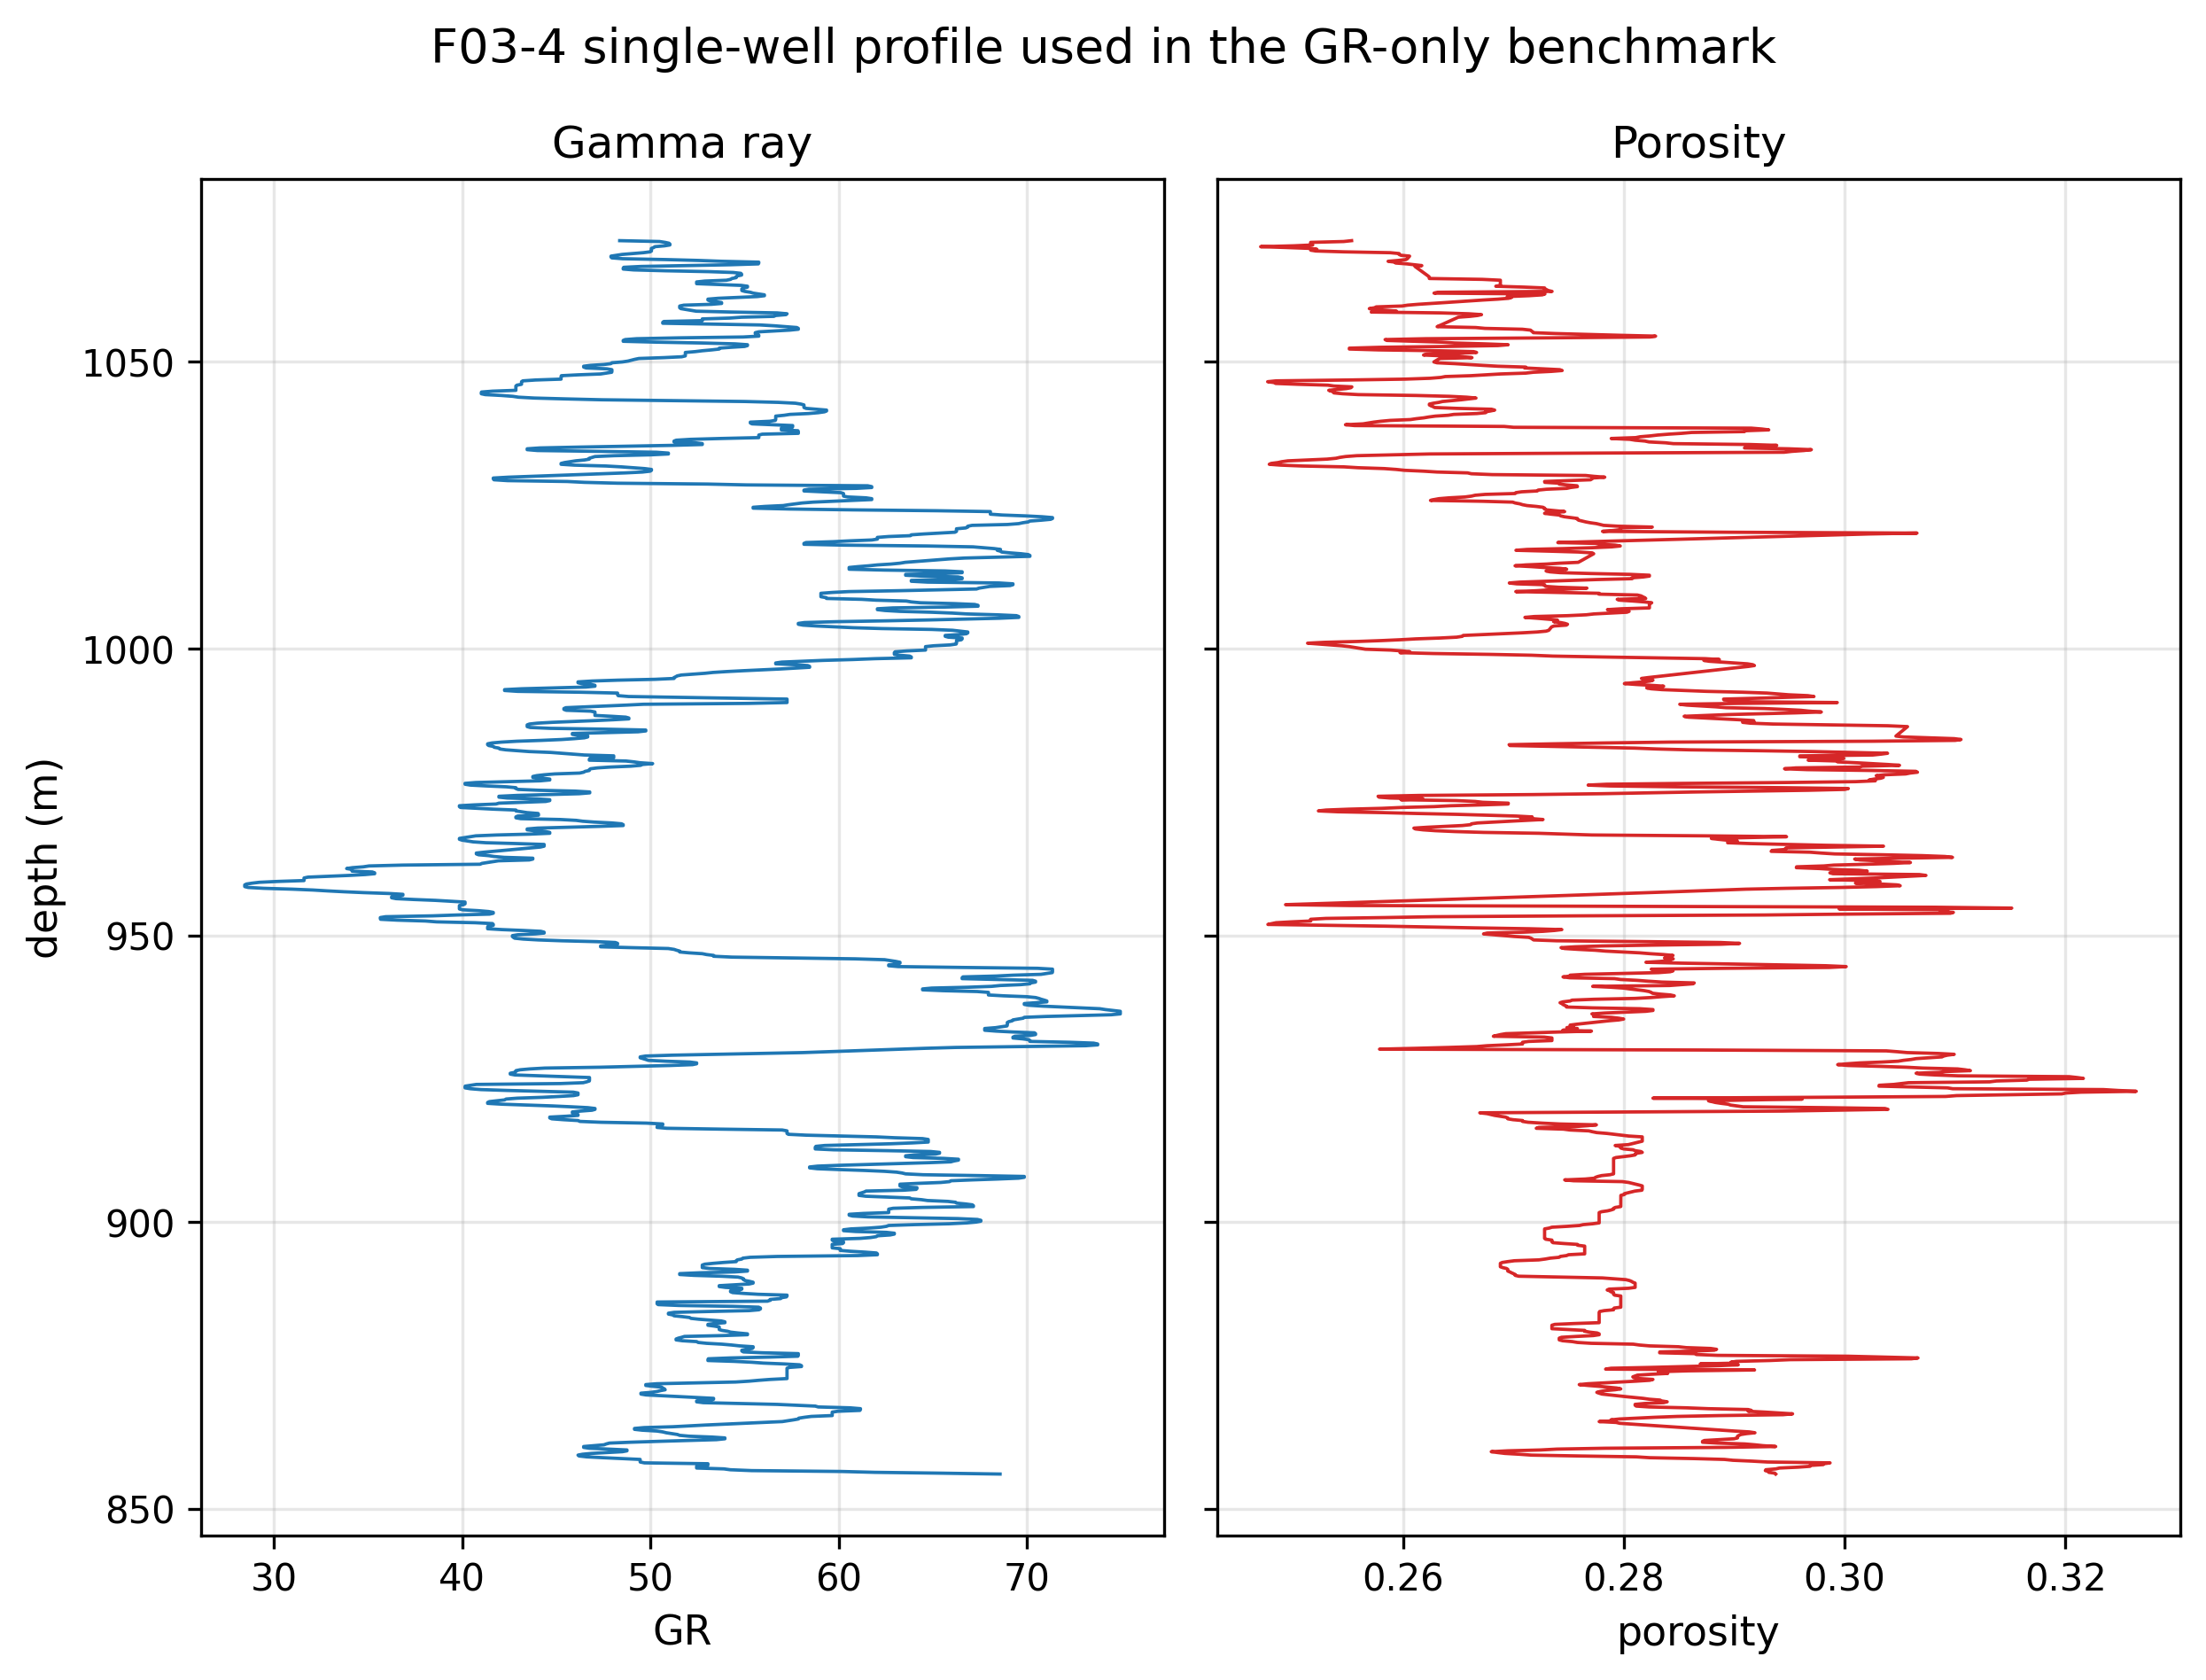
\includegraphics[width=0.54\linewidth]
    {eda_f03_gr_porosity_depth.png}
    \caption{F03-4 depth profiles used in the gamma-ray-only (GR-only)
    porosity benchmark. Gamma
    ray is the only dense input, while porosity is reconstructed from the
    log-conditioned latent prior and sparse target observations.}
    \label{fig:eda_f03_profile}
\end{figure}

